% !TeX spellcheck = de_DE
\section{Malvér a spôsoby ukrytia malvéru}
\noindent
\subsection{Malvér}
\noindent Je to softvér, ktorého cieľom je poškodiť, zablokovať, zmocniť sa alebo odcudziť dôležité informácie uložené v počítači. Cieľom malvéru je získať informácie pre útočníka a následné zneužitie informácií na rôzne druhy nelegálnej činnosti za účelom danej obete uškodiť alebo sa na nej finančne obohatiť. Malvér kedysi zahŕňal rôzne počítačové vírusy, backdoory, spyware, ramsomware a rôzne iné softvéry. V súčasnosti už toto delenie nie je aktuálne, pretože súčasné malvéry sú už kombináciou týchto vírusov a využívajú rôzne časti jednotlivých vírusov. V nasledujúcej časti kapitoly sa podrobnejšie budem zaoberať rôznymi spôsobmi ukrytia malvéru, ktoré môžu byť v súčasnosti využívané na ukrytie malvéru. 

\subsection{DLL Injection / Reflective DLL Injection}
\noindent DLL Injection je technika používaná na ukrytie funkcie na spustenie malvéru vo vnútri iného programu. Najčastejšie sa na to využíva alokovaná pamäť vyhradená pre beh infikovaného programu, kde sa funkcia na spustenie malvéru ukryje a pre antivírusové programy je ťažko detekovateľná. Po nakopírovaní DLL funkcie do alokovanej pamäte iného programu môže byť následne vyvolané spustenie infikovaného programu a spolu s ním aj spustenie malvéru. Hlavným cieľom DLL Injection je škodlivý kód ukryť do oficiálneho alebo overeného programu, kde je malvér ukrytý pred antivírovým softvérom, odkiaľ môže byť následne spustený.

\subsection{Process hollowing}
\noindent Proces Hollowing využíva rovnaké alebo podobné princípy ukrývania škodlivého softvéru ako DLL Injection. Cieľom je schovať škodlivý kód do existujúce programu z ktorého sa po spustení, spustí aj volanie škodlivého malvéru.  Oproti DLL Injection ide ale ukrytie malvérového programu do iného programu. Malvér si podľa potreby alokuje virtuálnu pamäť  v pamäti iného programu. Po spustení infikovaného programu malvér pozastaví thread v ktorom program beží, následne zmení obsah legitímneho súboru zmapovaním pamäte cieľového procesu. Po zmapovaní uvoľní všetku pamäť programu a alokuje pamäť pre malvér a zapíše každú z častí malvéru do cieľovej pamäte programu. Malvér volá SetThreadContext, aby ukazoval vstupný bod na novú časť kódu, ktorú napísal. Na konci malvér obnoví pozastavený thread volaním ResumeThread, aby sa proces dostal z pozastaveného stavu a nasledovným spustením programu umožní získavanie údajov.

\subsection{Thread Execution Hijacking }
\noindent Táto technika ukrytia malvéru spočíva v napojení sa na už existujúci thread vyvolaný iným programom. Po získaní prístupu do threadu malvér uvedie thread do pozastaveného režimu aby vykonal vloženie volania škodlivého malvéru do threadu iného procesu. Malvér si alokuje virtuálnu pamäť v programe a následne do tejto pamäte vloží škodlivý shell kód, ktorý obsahuje cestu k volaniu DLL so škodlivým malvérom.  Po vykonaní týchto úkonov, spustí pozastavený thread programu. Nevýhodou takéhoto spustenia pozastaveného programu je, že môže spôsobiť zlyhanie systému v rámci systémového volania. Preto aby sa tomu predišlo modernejší malvér proces ukončí a vyvolá ho znovu s už modifikovanou zmenou na infikovanie.

\subsection{Portable Executable Injection}
\noindent Výhodou tohto spôsobu ukrytia malvéru je využitie nakopírovania malvéru do už existujúceho bežiaceho procesu pomocou shell skriptu, ktorý vyvolá spustenie škodlivého malvéru. Namiesto toho aby proces prepisoval cesty volaním  DLL, táto technika zapisuje obsah malvéru priamo pomocou WriteProcessMemory. Počas doby zapisovania aby malvér nebol ľahko odhalený využíva vnorené cykly, ktoré spomaľujú systém buď diagnostikou alebo volaním zbytočných funkcií a snaží sa zahltiť systém a neumožniť skorú diagnostiku malvéru.  Keď malvér preformuluje všetky potrebné adresy, všetko, čo musí urobiť, je odovzdať jeho počiatočnú adresu CreateRemoteThread a nechať spustiť malvér.

\section{Aktuálne využívané malvéry}
\noindent Táto kapitola obsahuje opis jednotlivých malvérov používaných v roku 2019, ktoré boli detekované spoločnosťami ako Avast a McAfee. Tieto malvéry sú najčastejšie využívané v oblasti Európy. Kapitola obsahuje bližší opis malvérov, ich využitie, použité spôsoby úrokov a ukrytie malvéru v systéme.

\subsection{Sodinokibi}
\noindent Tento malvér bol detekovaný v období okolo apríla 2019. Patrí do rodiny ransomvéru, ktorých cieľom je šifrovať informácie v zariadení a následne za dešifrovanie pýta nemalý obnos peňazí. Názov bol objavený v hash kóde, ktorý obsahoval názov „Sodinokibi.exe“. vírus sa šíri sám zmeužívaním zraniteľnosti na serveroch Oracle WebLogic. Softvér je navrhnutý tak, aby rýchlo vykonával šifrovanie definovaných súborov v konfigurácii ransomvéru. Prvou akciou škodlivého softvéru je získať všetky funkcie potrebné pri  behu programu a vytvoriť dynamický IAT, ktorý sa pokúsi zahltiť volanie systému Windows statickou analýzou. Po zahltení systému dôjde k spusteniu malvéru. Technika využívaná na ukrytie malvéru je Portable Executable Injection ktorú volá po spomalení RunPE na jej spustenie z pamäte. táto technika ukrytia malvéru je opísaná v predošlej kapitole. Analýza spoločnosti McAfee ukazuje podobnosť s iným starším malvérom GandCrab.(pridať odkaz na analýzu respektíve literatúru)

\subsection{Ryuk}
\noindent (nutné doplniť)

\subsection{Dharma}
\noindent (nutné doplniť)

\subsection{Muhstik}
\noindent (nutné doplniť)


\begin{table}[!htbp]
\begin{center}
\begin{tabular}{p{4cm}|c|c|c|c|c|c|c|c|c|c|c|c|c|c|c}
& \multicolumn{14}{c}%
	 {\textbf{Funkcia}}\\ \hline
&&&& & &\multicolumn{8}{c}%
	 {Modifikácia}\\ 
\textbf{Modul} &\begin{sideways} zobrazenie hlavièky \end{sideways} &\begin{sideways} blokovanie skriptov \end{sideways} &\begin{sideways} zmena IP \end{sideways} & \begin{sideways} zmena lokalizácie \end{sideways} & \begin{sideways} zmazanie/blokovanie cookies \end{sideways} & \begin{sideways} blokovanie trackerov \end{sideways}  & \begin{sideways} popis \end{sideways} & \begin{sideways}používate¾ský agent\end{sideways} & \begin{sideways} kódové oznaèenie prehliadaèa \end{sideways} & \begin{sideways} názov prehliadaèa \end{sideways} & \begin{sideways} verzia prehliadaèa \end{sideways} & \begin{sideways} platforma \end{sideways} & \begin{sideways} výrobca prehliadaèa \end{sideways} & \begin{sideways} oznaèenie výrobcu prehliadaèa \end{sideways} \\ \hline
User agent switcher & & & & & &  & X & X & X & X & X & X & X & X  \\ \hline
Ghostery &  && & & X & X &  &  & & & & & & \\  \hline
Better privacy && &  & & X &  &  &  & & & & & & \\  \hline
Anonymox &  && X & X & X &  & X & X & & & & & & \\  \hline
Modify headers & & &  &  & X &  &  & X &  &  &  & & &  \\  \hline
Request policy & & &  &  & & X  &  &  &  &  &  & & &   \\  \hline
Live HTTP headers & X& &  &  & &  &  &  &  &  &  & & &   \\  \hline
User agent awitcher for chrome & & &  &  & &  & X & X &  &  &  & & &   \\  \hline
Header hacker & & &  &  & &  & X & X & X & X & X & X & X & X    \\  \hline
Mod header & & &  &  & &  & X & X & X & X & X & X & X & X    \\  \hline
Script no & &X &  &  & &  &  &  &  &  &  &  &  &     \\  \hline
No script & &X &  &  & &  &  &  &  &  &  &  &  &     \\  \hline
Proxify it & & &X  & X & &  &  &  &  &  &  &  &  &     \\  \hline
I'm not here & & &  & X & &  &  &  &  &  &  &  &  &     \\  \hline
Get anonymous personal edition & &X &X &X &X&X &  &  &  &  &  &  &  &     \\  \hline
Anonymous browsing toolbar & & & X & X & &  &  &  &  &  &  &  &  &     \\  \hline
Easy hide your IP and surf anonymously & & & X & X& &  &  & X & X & X & X &  &  &     \\  \hline
\end{tabular}
\caption{Moduly a ich funkcie pri anonymizácii}
\label{modulyVlastnosti}
\end{center}
\end{table}

\subsection{Anonymná sie}
\noindent Anonymná sie je sie serverov, medzi ktorými dáta prechádzajú šifrované. V anonymných sieach dáta prechádzajú z poèítaèa používate¾a, odkia¾ bola požiadavka poslaná, cez viaceré proxy smerovaèe, z ktorých každý správu doplní o smerovanie a zašifruje vlastným k¾úèom. Cesta od ...


\subsection{Funkcionalita}
\noindent  Rozšírenie tiež okrem splnenia špecifikácie malo pre preh¾adnos a overenie funkènosti zobrazova údaje, ktoré boli na server odoslané. Zoznam údajov odoslaných na server, sa mal uklada do krátkodobej histórie, aby nemal používate¾ k dispozícií len najnovšie údaje, ale aj údaje odoslané v nejakom èasovom období. 

\subsubsection{Funkcionalita2}
\noindent Samozrejmosou bolo nastavenie zapnutia rozšírenia pri štarte, prípadne interval zmeny odosielaných údajov.

\subsection{Vzh¾ad}
\noindent Dôležitou požiadavkou kladenou na rozšírenie bolo príjemné používate¾ské rozhranie. Z~tohto dôvodu malo rozšírenie obsahova zoznam modifikovaných vlastností a tlaèidlo pre prístup k nastaveniam rozšírenia v jednoduchej a praktickej forme. Predpokladaný vzh¾ad je zobrazený na obrázku è. \ref{vzhladobr}.
\begin{figure}[!htbp]
  \centering
  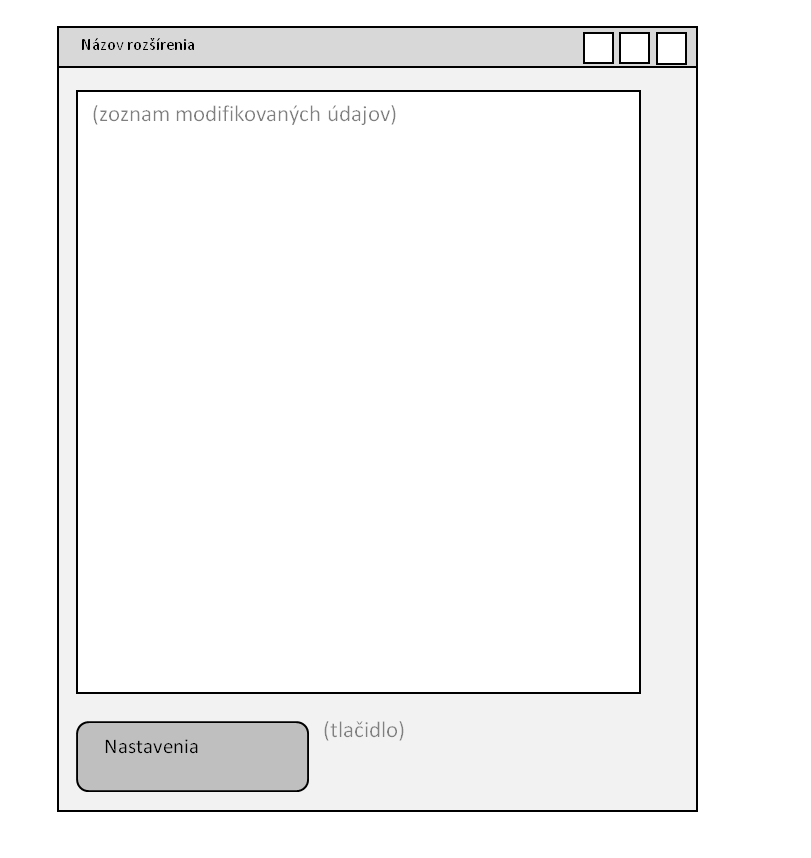
\includegraphics[width=8cm]{img/vzhlad.png}
  \caption{Predpokladaný vzh¾ad rozšírenia.}
  \label{vzhladobr}
\end{figure}	 
\noindent Dôležitou požiadavkou kladenou na rozšírenie bolo príjemné používate¾ské rozhranie.\cite{anonlib} Z~tohto dôvodu malo rozšírenie obsahova zoznam modifikovaných vlastností a tlaèidlo pre prístup k nastaveniam rozšírenia v jednoduchej a praktickej forme. Predpokladaný vzh¾ad je zobrazený na obrázku è. \ref{vzhladobr}.

\begin{algorithm}
\lstset{
    language=C,
    basicstyle=\small\sffamily,
    frame=none,
    numbers=left,
    xleftmargin=5.0ex,
    numberstyle=\tiny,
    stepnumber=1,
    showstringspaces=false,
    keywordstyle=\color{blue}\bfseries
    }
\lstset{emph={%  Adjust any special keywords
    printf%
    },emphstyle={\color[rgb]{1,0,0}\bfseries}%
}%
\begin{lstlisting}
/* Hello World program */

#include<stdio.h>

struct cpu_info {
    long unsigned utime, ntime, stime, itime;
    long unsigned iowtime, irqtime, sirqtime;
};

main()
{
    printf("Hello World");
}\end{lstlisting}
 \caption{Ukážka algoritmu}
 \label{euclid}
\end{algorithm}